% The FCal is the final part of the calorimeter system and is located between the end-cap calorimeters and the beam pipe. It covers the psuedorapidity of $3.1 < |\eta| < 4.9$ and is composed of three longitudinal sections: FCal1, FCal2, and FCal3 as shown in Figure~\ref{fig:forward_detector_layout}. 

% \begin{figure}[htp]
%     \centering
%     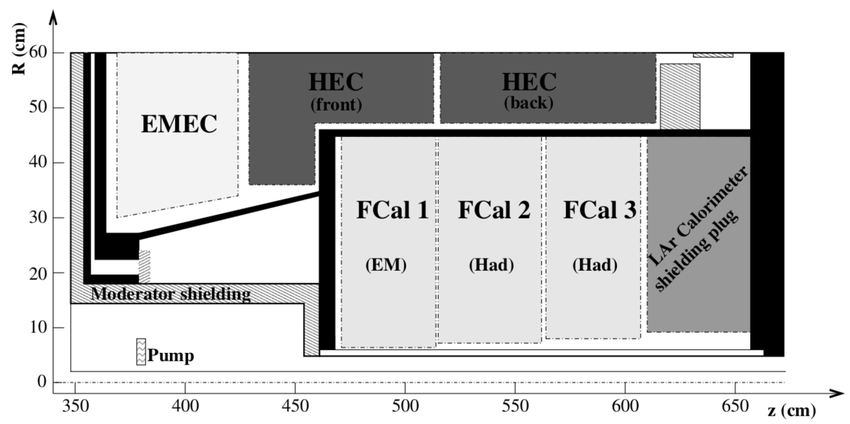
\includegraphics[width=0.8\textwidth]{figures/atlas/atlas_fcal_breakdown.png}
%     \caption{The layout of the forward calorimeter system. Depicted are the three different layers with the FCal1 being a ECal, while the FCal2 and FCal3 are HCals. Taken from~\cite{atlas_collaboration_paper}}\label{fig:forward_detector_layout}
% \end{figure}

% FCal1 is a LAr based ECal, that uses copper absorber material to optimize both heat removal and energy resolution. It provides a total of 27.6 \radlength{}. The structure consists of longitudinally stacked copper plates with holes drilled in them for the electrodes. Each electrode is co-axial structure consisting of an inner copper rod and an outer copper tube, separated by a plastic fiber containing the liquid argon. The electrode structure can be seen in Figure~\ref{fig:atlas_fcal_electrode}. 

% \begin{figure}[htp]
%     \centering
%     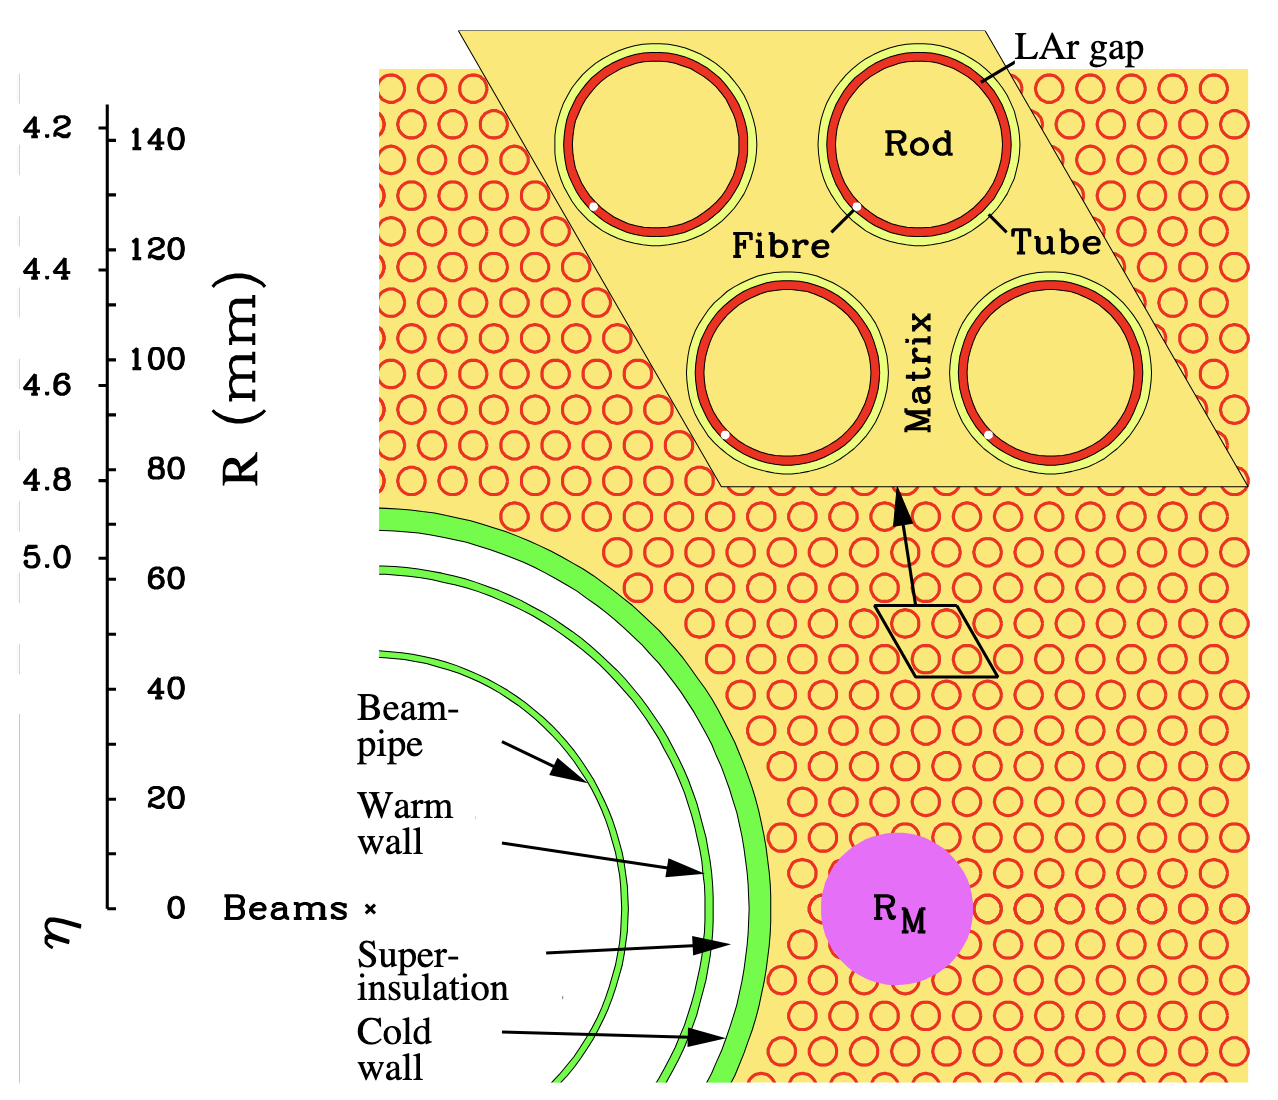
\includegraphics[width=0.6\textwidth]{figures/atlas/atlas_fcal_electrode.png}
%     \caption{Electrode structure with FCal1 with the matrix of copper plates and copper tubes. This figure also applies to FCal2 and FCal3 with the copper rods being replaced with tungsten rods. Taken from~\cite{atlas_collaboration_paper}}\label{fig:atlas_fcal_electrode}
% \end{figure}

% FCal2 and FCal3 are LAr based HCals, optimized for a high absorption length (3.68 \intlength{} and 3.60 \intlength{} respectively) by maximizing the amount of tungsten used in the modules. The modules are designed similarly to FCal1 with the only exception being that the rod is made of tungsten instead of copper. 

% To minimize contamination from unabsorbed particles in the muon system, a shielding plug is downstream from FCal3.


%%%%%%%%%%%%% revision

The FCal is the final part of the calorimeter system and is located between the end-cap calorimeters and the beam pipe covering $3.1 < |\eta| < 4.9$. It consists of three longitudinal sections: FCal1 (ECal), and FCal2/FCal3 (HCal) as shown in Figure~\ref{fig:forward_detector_layout}. 

\begin{figure}[htp]
    \centering
    \subfloat[Layout of the forward calorimeter system. FCal1 is an ECal; FCal2 and FCal3 are HCals.]{%
        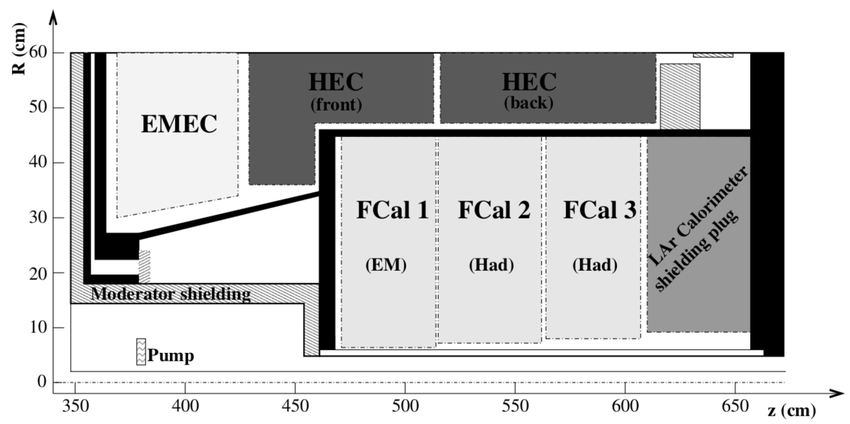
\includegraphics[width=0.55\textwidth]{figures/atlas/atlas_fcal_breakdown.png}\label{fig:forward_detector_layout}
    }
    \hfill
    \subfloat[Electrode structure shared across FCals. FCal2 and FCal3 use tungsten rods instead of copper.]{%
        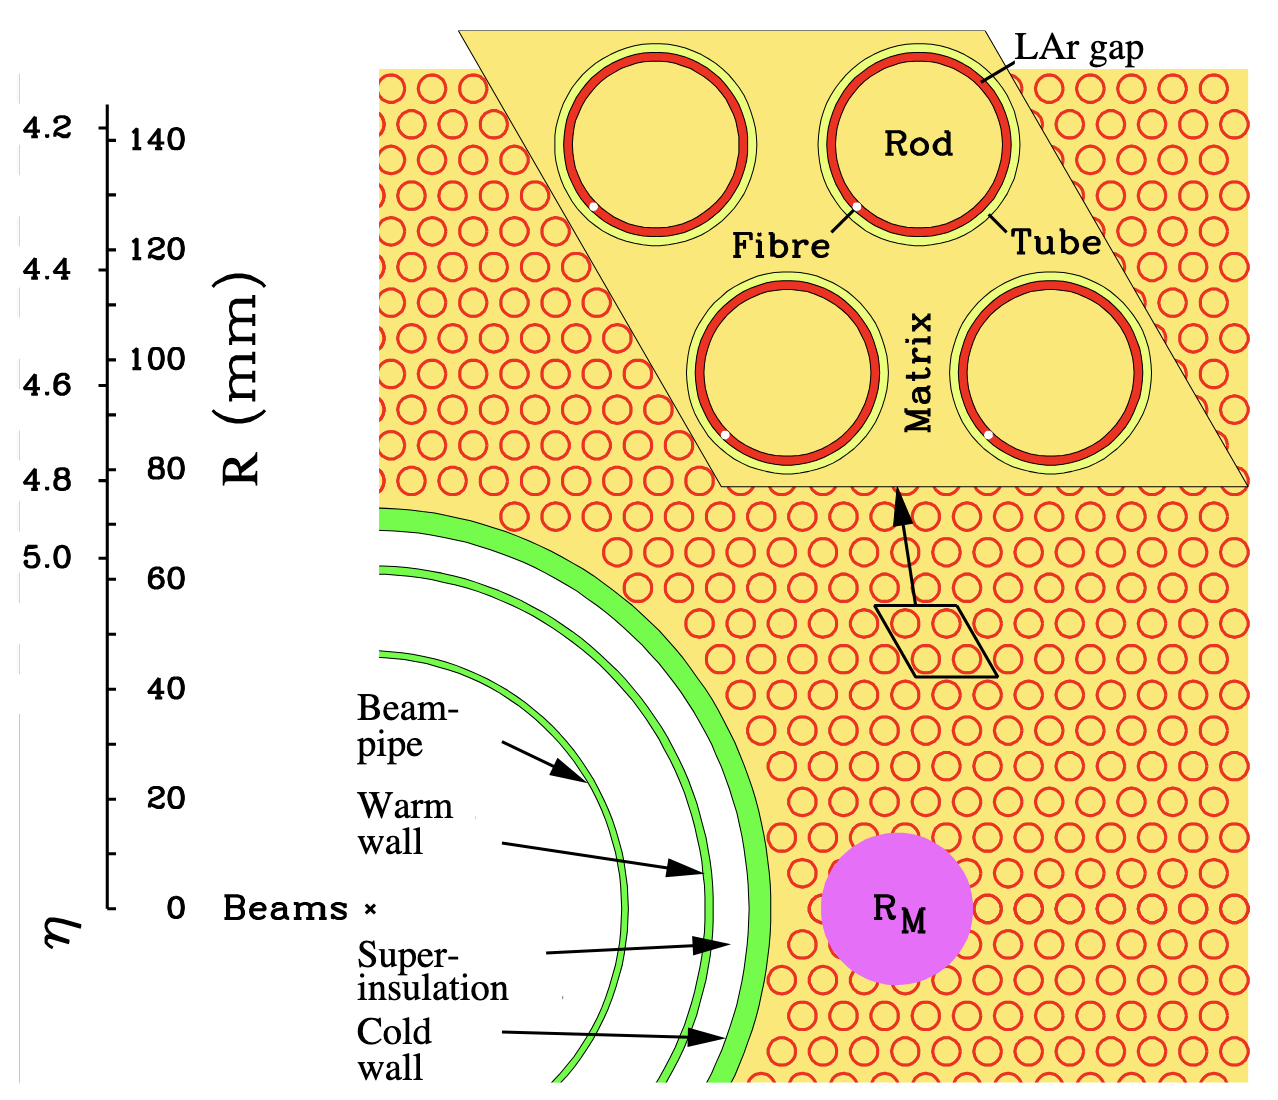
\includegraphics[width=0.4\textwidth]{figures/atlas/atlas_fcal_electrode.png}\label{fig:atlas_fcal_electrode}
    }
    \caption{Schematics of the forward calorimeter system (a) and the electrode structure common to all FCals (b). Figures from~\cite{atlas_collaboration_paper}.}\label{fig:atlas_fcal_combined}
\end{figure}

FCal1 uses copper absorbers and LAr as the active medium providing a total of 27.6 \radlength{}. It has stacked copper plates with co-axial electrodes made of an inner copper rod and an outer copper tube separated by a LAr-filled plastic fiber. The electrode structure is shared between all three FCals, and can be seen in Figure~\ref{fig:atlas_fcal_electrode}. 

FCal2 and FCal3 are optimized for a high absorption length (3.68 \intlength{} and 3.60 \intlength{} respectively) by using tungsten rods in the modules instead of copper. A shielding plug is placed downstream of FCal3 to reduce leakage into the muon system.
